\section{Previous work} \label{tex:previous_work}
In this section a recap of some different approaches to speed up or decrease the number of parameters will be given. In 2013 Denil et al. found NNs to be heavily over-parametrized \cite{Denil2013}. They did this by training only a fraction of the weights and using these to predict the rest of the weights. They reported that in some cases more than 95\% of the weights could be predicted, hence would not need to be learned. Ever since, numerous attempts have been proposed to optimise the evaluation time and number of parameters in NNs. One approach have been to decompose the dense layer of a NN, an other have tried speeding up the evaluation of a convolution, and some have had success in decomposing and speeding up an entire network. All the work described below follow approximately the same structure:

\begin{enumerate}
    \item \textbf{Decompose weights of pre-trained NN} Using some specific algorithm to get a smaller representation of the weights or filters
    \item \textbf{Changing the evaluation algorithm} In order for it to correspond to original evaluations and in order to do back-propagation
    \item \textbf{Fine-tuning} Which is training the network using the new algorithm and back-propagation 
\end{enumerate}
Some approaches will be discussed in the following. In the end the methods will be compared using a set of different metrics. 

\subsection{Decomposing the dense layer}
In 2015 Nokinov et al. used TT-decomposition to decompose the weights of a dense (fully-connected) layer in an ANN\cite{Novikov2015}. This method exploits the power of the dense layer and allows it to have a big amount of neurons. The dense layer performs a linear transformation on an input vector $\bs{x}$ of dimension $N$:
\begin{equation}
    \bs{y} = \bs{W} \bs{x} + \bs{b}
    \label{eq:linearTransform}
\end{equation}
Where $\bs{W} \in \R^{M\times N}$ is the weight matrix and $\bs{b} \in \R^{M}$ is the bias vector. $M$ is the dimension of the output $\bs{y}$. Since the weights of the dense layer are given in a matrix, Nokinov et al. folds this matrix into a 3-dimensional tensor in order to decompose it using the TT algorithm. They define the TT-layer to be the same transformation but with the weights stored in the TT-format. Let $\tensor{X}$ be the input tensor of dimension $d$ (formed from $\bs{x}$), and let the decomposition of the weight matrix have cores $\bs{G}_k[i_k, j_k]$. In the TT-layer the transformation corresponding to \eqref{eq:linearTransform} is given as:
\begin{equation}
    \tensor{Y}(i_1, i_2, \dots, i_d) = \sum_{j_1, j_2, \dots, j_d} \bs{G}_1[i_1, j_1] \bs{G}_2[i_2, j_2]\dots \bs{G}_d[i_d, j_d] \tensor{X}(j_1, j_2, \dots j_d) + \tensor{B}(i_1, i_2, \dots, i_d)
\end{equation}
Where $\tensor{B}$ is the bias tensor. The properties of the TT-format allows for computation of back-propagation, which is then used for fine-tuning the network. The authors report a best-case compression of a dense layer of up to 200,000 times and of a whole network of up to 7.

\subsection{Speeding up the evaluation of a convolution}
In 2013 Rigamonti et al. \cite{Rigamonti2013} found that filters can be computed as a linear combination of smaller separable filters. A filter is called separable when it can be expressed using multiple parts of lower dimension, as for instance using the CP-decomposition as illustrated by \cite{Sironi2015} in \autoref{fig:separable_filters}. Ever since many approaches have been considered using this principle in different ways. For instance Lebedev et al. using CP-decomposition in \cite{Lebedev2015}, while Jaderberg et al. proposed two different schemes for using rank-1 filters to exploit the cross-channel / filter redundancy \cite{Jaderberg2014}. 

\begin{figure}[]
    \centering
    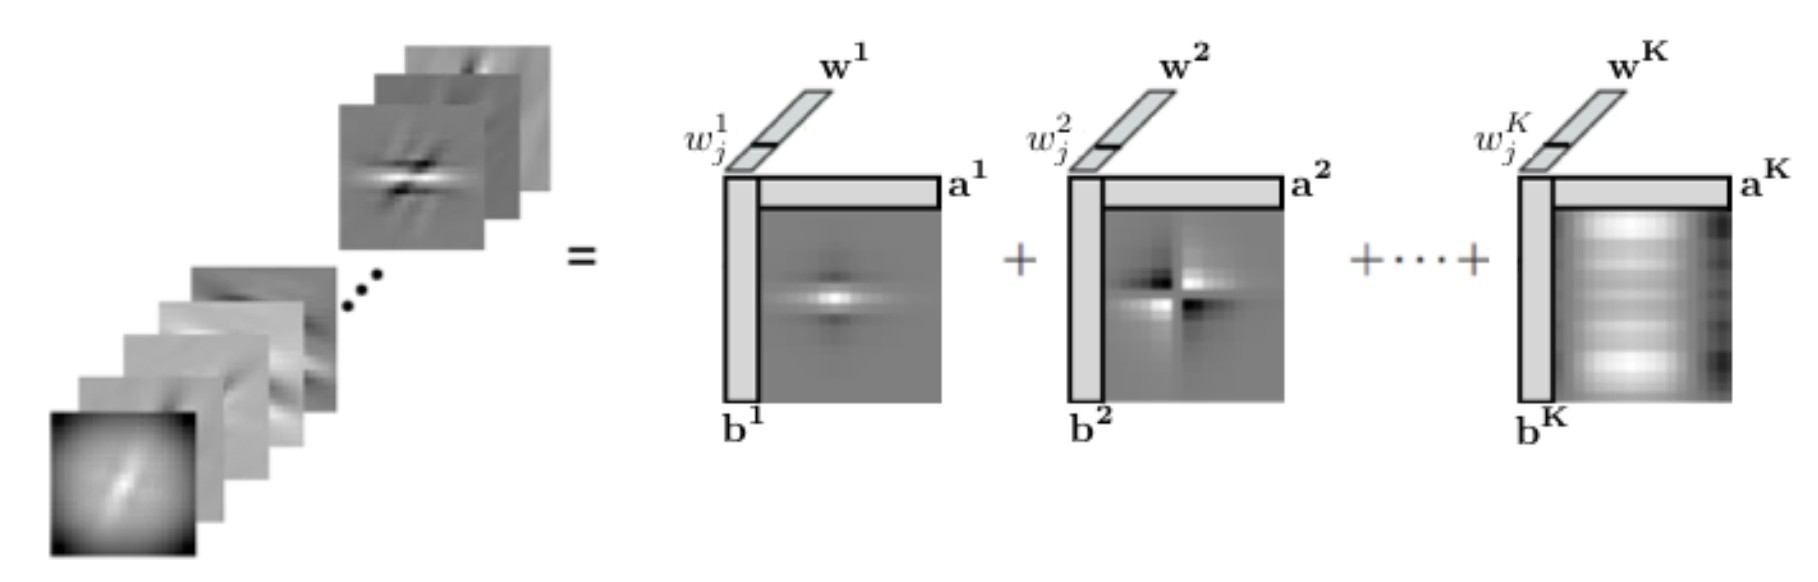
\includegraphics[width=.8\linewidth]{Pics/02_Previous_work/separable_filters.png}
    \caption{Taken from \cite{Sironi2015}. Left: A bank of two-dimensional filters is stacked together to form a 3-dimensional tensor. Right: The tensor is decomposed in the sum of $K$ rank-one tensors. Thus, the original filters are approximated by the weighted sum of the separable filters $s_k = \boldsymbol{a}_k \circ \boldsymbol{b}_k$}
    \label{fig:separable_filters}
\end{figure}

\subsubsection{Convolution using CP-decomposition}



% Outline:
% Speeding up the dense layer
% Speeding up the convolutional layer
% Speeding up the entire network